\documentclass[notitlepage]{simple}

\usepackage{float}
\usepackage{pgf,tikz}
\usepackage{mathrsfs}
\usetikzlibrary{arrows}

\definecolor{uuuuuu}{rgb}{0.26666666666666666,0.26666666666666666,0.26666666666666666}
\definecolor{xdxdff}{rgb}{0.49019607843137253,0.49019607843137253,1.}
\definecolor{qqqqff}{rgb}{0.,0.,1.}

\author{Matt McCarthy}
\title{How To Git}
\date{CNU FOSS Day\\ 12 March, 2016}

\begin{document}

\maketitle

\section{Version Control}

% TODO: Get the information to put here.

\section{Git 101}

Before starting, make sure your terminal is open.

To start, we need to configure Git.
To do so, we run the following two commands.
\begin{terminal}
	\verb|git config --global user.name "Your Name Here"|\\
	\verb|git config --global user.email "your.email@host.domain"|
\end{terminal}
These commands tell our Git installation who we are and how to contact us so that other users know who is responsible for each commit.

\subsection{Local Git}

Our first task is to make a repository on our local machine.
Next we want a directory in which we will store our Git repositories.
For the sake of simplicity, let's just make a new folder in the home directory called \verb|git| and then enter that directory, that is run the following.
\begin{terminal}
	\verb|mkdir ~/git|\\
	\verb|cd ~/git|
\end{terminal}
Next we want to actually make the repository.
To do so, we want to make a folder for the repository (\verb|mkdir my-git-repo|) and then enter that folder (\verb|cd my-git-repo|).
We will now turn this folder into a Git repository by running
\begin{terminal}
	\verb|git init|
\end{terminal}
which creates the directories and files necessary to make a folder a Git repository.

We're now going to start making changes, tracking them, and committing them.
Let's begin by creating a file and telling Git to track it.
Run
\begin{terminal}
	\verb|touch file.txt|
\end{terminal}
this will create a file called \verb|file.txt|.
If we run
\begin{terminal}
	\verb|git status|
\end{terminal}
it will list \verb|file.txt| as an untracked file.
We now need to run
\begin{terminal}
	\verb|git add .|
\end{terminal}
which tracks all untracked files and tracks any changes you made.
If we run \verb|git status| again, we will see that \verb|new file: file.txt| is in the list of changes to be committed.
Lastly, to commit our changes, we run
\begin{terminal}
	\verb|git commit -m "Added file.txt"|
\end{terminal}
which logs our changes and gives us a point to which we can revert.
If we run \verb|git status| once more, it will report that there is nothing to commit and that the working directory is clean.
The \verb|git add .| and \verb|git commit -m "message here"| commands define the workflow on a single machine, that is these commands track and log each change you make to your project.

Next we'll make some changes to the project and then reset them.
For now, run the following command.
\begin{terminal}
	\verb|echo "Subversion is the best version control software" > file.txt|
\end{terminal}
Then track the change using \verb|git add .| but don't commit the change just yet.
Run \verb|git status| and ensure that the change is tracked.
You see, the statement we piped into \verb|file.txt| is a lie and so we need to undo the change even though we just tracked it.
To do so, we run
\begin{terminal}
	\verb|git reset --hard|
\end{terminal}
Now run \verb|git status| to make sure the change is gone.
More generally, we can run \verb|git reset --hard commit-id| to reset to any given commit.
Since the old statement is gone, we will go ahead and pipe the correct statement into \verb|file.txt|.
\begin{terminal}
	\verb|echo "git is the best version control software" > file.txt|
\end{terminal}
We will now track and commit our changes in one command by running
\begin{terminal}
	\verb|git commit -am "Did a thing"|
\end{terminal}
which adds all changes in \textit{tracked} files and then commits them in one fell swoop.
Furthermore, it does not add any untracked files, so any new files would be skipped by this command.

\begin{figure}[H]
	\centering
	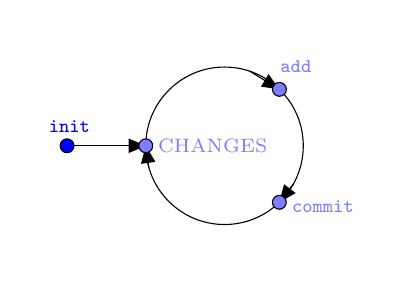
\begin{tikzpicture}[line cap=round,line join=round,>=triangle 45,x=1.0cm,y=1.0cm]
	\clip(0.5,0.5) rectangle (5.,3.5);
	\draw(3.,2.) circle (1.cm);
	\draw [->] (1.,2.) -- (2.,2.);
	\draw [->] (3.3186394600941354,2.9478759910826513) -- (3.6974712186505396,2.716612795834774);
	\draw [->] (3.872945513982138,1.5121822782857706) -- (3.696276389206922,1.2822262265637097);
	\draw [->] (2.039158952729161,1.7228998703005047) -- (2.,2.);
	\begin{scriptsize}
	\draw [fill=qqqqff] (1.,2.) circle (2.5pt);
	\draw[color=qqqqff] (1.0299173553719023,2.25) node {\verb|init|};
	\draw [fill=xdxdff] (2.,2.) circle (2.5pt);
	\draw[color=xdxdff] (2.85,2.) node {CHANGES};
	\draw [fill=xdxdff] (3.696276389206922,1.2822262265637097) circle (2.5pt);
	\draw[color=xdxdff] (4.25,1.221983471074382) node {\verb|commit|};
	\draw [fill=xdxdff] (3.6974712186505396,2.716612795834774) circle (2.5pt);
	\draw[color=xdxdff] (3.905950413223143,3.007107438016532) node {\verb|add|};
	\end{scriptsize}
	\end{tikzpicture}
	\caption{Workflow for Git on a single machine}
\end{figure}

\subsection{Using GitHub}

Now that we know how to deal with changes in a project locally, we're going to bring GitHub into the picture.
To begin, if you do not have a GitHub account create one at \url{github.com}.
Continuing with our toy project, create a repository on your GitHub account by clicking the `New repository' button.
\begin{figure}[H]
	\centering
	% TODO: Add picture
	\caption{The `New repository' button}
\end{figure}
For the name, call it \verb|my-git-repo| and then create the repository.
This should bring you to webpage of your new repository.
From here copy the URL next to the `Download ZIP' button.
\begin{figure}[H]
	\centering
	% TODO: Add picture
	\caption{Click here}
\end{figure}
Our next step is to add the GitHub repository as a remote server.
To do so run
\begin{terminal}
	\verb|git remote add origin copied-url|
\end{terminal}
which adds a place from which Git can fetch code for this repository.
Now that we have added the server, run
\begin{terminal}
	\verb|git push origin master|
\end{terminal}
to push your changes to GitHub.
The \verb|git push| command requires both a place to which it can push as well as a \textit{branch} to which we can push.
The default branch of any Git repository is called the master branch.
If you want to learn more about branching, check out the advanced Git section of this paper after you finish the demo.

Now that your project is on GitHub run \verb|cd ..| to go into the parent directory and then delete your project using
\begin{terminal}
	\verb|rm -rf my-git-repo|
\end{terminal}
We will now \textit{clone} the repository from the GitHub URL.
Now run
\begin{terminal}
	\verb|git clone copied-url|
\end{terminal}
which creates a directory for your project and then copies all of the project's files into that directory.
To check run \verb|cd my-git-repo| and then
\begin{terminal}
	\verb|cat file.txt|
\end{terminal}
and it should output the contents of the file.

When we use a \verb|git| server, the workflow will change a little bit.
Instead of just running \verb|git add| and \verb|git commit|, we now have to run \verb|git push| in order to push our commits to the server.
Furthermore, instead of running \verb|git init|, we can just create an empty repository on the server and then use \verb|git clone| to set it up on our machine.

Lastly, GitHub has a Git cheat sheet at
\begin{center}
\url{https://training.github.com/kit/downloads/github-git-cheat-sheet.pdf}
\end{center}
if you wish to have a quick reference document.

\begin{figure}[H]
	\centering
	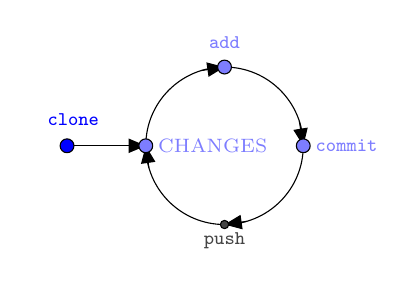
\begin{tikzpicture}[line cap=round,line join=round,>=triangle 45,x=1.0cm,y=1.0cm]
	\clip(0.5,0.5) rectangle (5.,3.5);
	\draw(3.,2.) circle (1.cm);
	\draw [->] (1.,2.) -- (2.,2.);
	\draw [->] (2.7062144040845406,2.955871342614998) -- (3.,3.);
	\draw [->] (3.9502651794615264,2.3114419507756674) -- (4.,2.);
	\draw [->] (2.039158952729161,1.7228998703005047) -- (2.,2.);
	\draw [->] (3.2799698178262338,1.0399911973808025) -- (3.,1.);
	\begin{scriptsize}
	\draw [fill=qqqqff] (1.,2.) circle (2.5pt);
	\draw[color=qqqqff] (1.0795041322314065,2.3294214876033084) node {\verb|clone|};
	\draw [fill=xdxdff] (2.,2.) circle (2.5pt);
	\draw[color=xdxdff] (2.85,2.0) node {CHANGES};
	\draw [fill=xdxdff] (4.,2.) circle (2.5pt);
	\draw[color=xdxdff] (4.55,2) node {\verb|commit|};
	\draw [fill=xdxdff] (3.,3.) circle (2.5pt);
	\draw[color=xdxdff] (3,3.304628099173557) node {\verb|add|};
	\draw [fill=uuuuuu] (3.,1.) circle (1.5pt);
	\draw[color=uuuuuu] (3,0.8) node {\verb|push|};
	\end{scriptsize}
	\end{tikzpicture}
	\caption{Workflow for Git with a Git server}
\end{figure}

\section{Git Demonstration}

For our demonstration, we will make a few classes that could be used for auto insurance.

\subsection{Forking the Demo}

In your web browser, navigate to \url{https://github.com/matt-mccarthy/cnu-foss-day-demo}.
Once the page has loaded look for a button called `Fork' and click it in order to fork the repository.
\begin{figure}[H]
	\centering
	% TODO: Add picture
	\caption{The Fork button}
\end{figure}
After that you should be on the page for your forked repository.
From here, clone your repository and then in your terminal use \verb|cd| to enter the repository's directory.
Once you have \verb|cd|'d into the repository, run the following command.
\begin{terminal}
	\verb|git remote add upstream https://github.com/matt-mccarthy/cnu-foss-day-demo.git|
\end{terminal}
This will allow you to pull changes from the original repository into your own.

\subsection{Claiming and Fixing an Issue}

% TODO: Claim issue.

Once you have your issue claimed, open the file that to which the issue applies and add the code necessary to fix the issue.
Once you fix your issue, you can move on to the next section.

\subsection{Pull Changes from Upstream}

Now that you have fixed your issue, go ahead and push your changes to your repository.
After you have done that, run the command
\begin{terminal}
	\verb|git pull upstream master|
\end{terminal}
pulls any changes from the original repository (called \verb|upstream|) into your local repository and then \textit{merges} them into your code
(if you want to learn more about merging and branching check out the Advanced Git section of this paper).
Sometimes, the merge operation will require manual intervention in order to succeed, but this should not be the case for this demo.
Once you successfully merge, run \verb|git status| to ensure you do not need an extra commit, and then push your changes to your repository.
If you do need an extra commit, commit your changes and then push.

\subsection{Pull Requests}

Now that your fork is up to date, we will start talking about creating a pull request.
Navigate to the GitHub page for your repository and click the ``New pull request'' button.
\begin{figure}[H]
	\centering
	% TODO: Add picture
	\caption{Pull request button}
\end{figure}
Quickly inspect the options.
\begin{figure}[H]
	\centering
	% TODO: Add picture
	\caption{Proper set up}
\end{figure}
The ``base fork'' field should be set to \verb|matt-mccarthy/cnu-foss-day-demo| with ``base'' \verb|master|.
The ``base fork'' field tells GitHub where we want to merge our changes, and the ``base'' field specifies a branch to merge.
Furthermore, if you look at the ``head fork'' field you should see your repository listed there and again with the ``compare'' field set to \verb|master|.
For our purposes, GitHub did all of the work and so we can go ahead and click the ``Create pull request'' button.
And that's the last step for you to do.
All that is left is for your request to be approved or denied.

\begin{figure}[H]
	\centering
	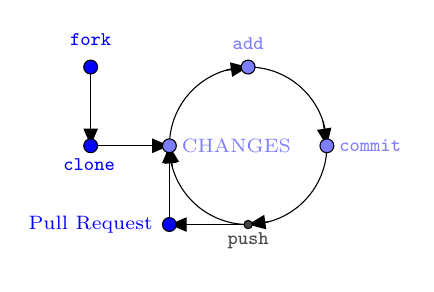
\begin{tikzpicture}[line cap=round,line join=round,>=triangle 45,x=1.0cm,y=1.0cm]
	\clip(0.2,0.5) rectangle (5.,3.5);
	\draw(3.,2.) circle (1.cm);
	\draw [->] (1.,2.) -- (2.,2.);
	\draw [->] (2.7062144040845406,2.955871342614998) -- (3.,3.);
	\draw [->] (3.9502651794615264,2.3114419507756674) -- (4.,2.);
	\draw [->] (2.039158952729161,1.7228998703005047) -- (2.,2.);
	\draw [->] (3.2799698178262338,1.0399911973808025) -- (3.,1.);
	\draw [->] (1.,3.) -- (1.,2.);
	\draw [->] (3.,1.) -- (2.,1.);
	\draw [->] (2.,1.) -- (2.,2.);
	\begin{scriptsize}
	\draw [fill=qqqqff] (1.,2.) circle (2.5pt);
	\draw[color=qqqqff] (0.9803305785123981,1.7674380165289278) node {\verb|clone|};
	\draw [fill=xdxdff] (2.,2.) circle (2.5pt);
	\draw[color=xdxdff] (2.85,2.0) node {CHANGES};
	\draw [fill=xdxdff] (4.,2.) circle (2.5pt);
	\draw[color=xdxdff] (4.55,2) node {\verb|commit|};
	\draw [fill=xdxdff] (3.,3.) circle (2.5pt);
	\draw[color=xdxdff] (3,3.3) node {\verb|add|};
	\draw [fill=uuuuuu] (3.,1.) circle (1.5pt);
	\draw[color=uuuuuu] (3,0.8) node {\verb|push|};
	\draw [fill=qqqqff] (1.,3.) circle (2.5pt);
	\draw[color=qqqqff] (1.,3.35) node {\verb|fork|};
	\draw [fill=qqqqff] (2.,1.) circle (2.5pt);
	\draw[color=qqqqff] (1.,1.) node {Pull Request};
	\end{scriptsize}
	\end{tikzpicture}
	\caption{Workflow for a typical FOSS project using GitHub}
\end{figure}

\section{Advanced Git}

In this section, we will cover branches, tags, and the \verb|.gitignore| file.

\subsection{Branches}

So far in this demo, we have done all of our work in a branch called master, however this is typically not the best way to do things.
The more usual workflow involves creating either a branch for a new feature or release.
These branches can operate independent of all other branches, which makes it easier to tackle an issue or add a new feature since the base code does not change until you decide to bring those changes in.

To start, lets see how branches work.
In the demo repository, run
\begin{terminal}
	\verb|git checkout testing|
\end{terminal}
which switches the branch from master to the testing branch.
For this excercise, implement the \verb|toString()| function in \verb|Car.java|.

After that's done, we need to merge the changes you did in master into testing.
To do so, we run
\begin{terminal}
	\verb|git merge master|
\end{terminal}
which merges all changes you made on master into the testing branch, a necessary step to enable what we call a \textit{fast-forward} merge when we go back into master.

Once it merges, run \verb|git status| to make sure you do not need an extra commit to finish the merge.
Now run
\begin{terminal}
	\verb|git push origin testing|
\end{terminal}
to push the latest commits in the testing branch to GitHub.
Now that we have brought testing up to speed, use
\begin{terminal}
	\verb|git checkout master|
\end{terminal}
to switch back to the master branch.
Now we run
\begin{terminal}
	\verb|git merge testing|
\end{terminal}
in order to merge our testing changes into master.
Once we have everything merged into master, run
\begin{terminal}
	\verb|git push origin master|
\end{terminal}
in order to push your changes to master.

Next, run
\begin{terminal}
	\verb|git checkout -b person-toString|
\end{terminal}
which creates a new branch called \verb|person-toString| and immediately switches to it.
For this part create a method \verb|public String toString()| for the person class that returns a string in the format \linebreak\verb|lastname, firstname|.
Once you have it implemented commit and then run
\begin{terminal}
	\verb|git push origin person-toString|
\end{terminal}
which will push the \verb|person-toString| branch to GitHub.
Next switch to the master branch by running
\begin{terminal}
	\verb|git checkout master|
\end{terminal}
and then run
\begin{terminal}
	\verb|git merge person-toString|
\end{terminal}
which will merge the \verb|person-toString| branch into master.
Now push your master branch to GitHub by running \verb|git push origin master|.

\subsection{Tags}

Git also a tag feature that is typically used to denote releases.
For example, if you were to run
\begin{terminal}
	\verb|git checkout v0.1beta2|
\end{terminal}
your local repository would look like how it did when you first cloned it.
This is because that tag marks the commit that represents the initial version of the repository.
What you need to do now is run
\begin{terminal}
	\verb|git tag release1|
\end{terminal}
in order to easily switch to the current state of the repository.
Once you have made your tag, go ahead and run
\begin{terminal}
	\verb|git checkout v0.1beta2|
\end{terminal}
which brings you back to the way your repository originally was.
Run
\begin{terminal}
	\verb|git checkout release1|
\end{terminal}
in order to get back to release1.

Once you are back at release1, run
\begin{terminal}
	\verb|git push origin release1|
\end{terminal}
which pushes the tag to the Git server, since git push does not push tags unless you tell it to do so.

\subsection{\texttt{.gitignore}}

In the demo repository, you may have seen an odd file entitled \verb|.gitignore|.
This file tells Git which files to ignore.
You can specify that certain file types should be ignored or you can actually spell out the files.
But this raises the question, what if you want to add an ignored file?
In this case we use the command
\begin{terminal}
	\verb|git add -f ignored_file_name_here|
\end{terminal}
which forces Git to track the ignored file.
If you want to generate a \verb|.gitignore| for your repository, an easy way to do so is to use \url{www.gitignore.io}.
This website takes the languages you are using and autogenerates a \verb|.gitignore| that ignores all of the typical temporary files that your languages produce.
For example, the \verb|.gitignore| for Java ignores \verb|.class| and \verb|.jar| files as well as JVM crash logs.

\end{document}
